\documentclass[acmtog]{acmart}
\usepackage{graphicx}
\usepackage{subfigure}
\usepackage{natbib}
\usepackage{listings}
\usepackage{bm}

\definecolor{blve}{rgb}{0.3372549 , 0.61176471, 0.83921569}
\definecolor{gr33n}{rgb}{0.29019608, 0.7372549, 0.64705882}
\makeatletter
\lst@InstallKeywords k{class}{classstyle}\slshape{classstyle}{}ld
\makeatother
\lstset{language=C++,
	basicstyle=\ttfamily,
	keywordstyle=\color{blve}\ttfamily,
	stringstyle=\color{red}\ttfamily,
	commentstyle=\color{magenta}\ttfamily,
	morecomment=[l][\color{magenta}]{\#},
	classstyle = \bfseries\color{gr33n}, 
	tabsize=2
}
\lstset{basicstyle=\ttfamily}

% Title portion
\title{Warm-up assignment:\\ {Programming simple graphics program with OpenGL}} 

\author{Name:\quad Haizhao Dai\\
student number:\ 2019533084\\
email:\quad daihzh@shanghaitech.edu.cn}

% Document starts
\begin{document}
\maketitle

\vspace*{2 ex}

\section{Introduction}
In this project, we will (1) load mesh objects from files and draw the meshes;
(2) render objects with a Phong lighting model; (3) manipulate a camera and control it.

\section{Implementation Details}
Here I will show how to make a bunny model step by step.

\subsection{Load mesh object and draw it}

\subsubsection{Load mesh data}
First step is to load the mesh data from the file. The format of file is given so I will not mention about that.
Notice that between each part of the data, there is one blank line. Using `std::getline' to handle it.
Also, all the data type (`float', `GLuint', `Vertex') are plain old data,
which indicates that allocate space for `std::vector' first is a preferable and fast way.

\subsubsection{Draw mesh}
Following with \href{LearnOpenGL.com}{LearnOpenGL}'s tutorial,
it is easy to draw mesh simply by creating vertex array objects(VAO),
vertex buffer objects(VBO) and putting data into OpenGL render pipeline.
As shown in fig.\ref{Bunny1}, with simple vertex shader and fragment shader,
I placed the bunny on the middle of the screen with proper size and used its vertex normals to generate color.
The result is shown later.

\subsection{Render objects with a Phong lighting model}
Phong lighting model consists of 3 kinds of lighting:
ambient, diffuse, specular. I decomposed and implemented them one by one.
This part of implementation is done in fragment shaders.

\subsubsection{Ambient lighting}
A simple model of global illumination, which imitates weak environment lighting.
So just a weak ambient strength is enough.
Ambient lighting is view-independent and light-sources-independent.

\subsubsection{Diffuse lighting}
Diffuse lighting creates a rough face for object just by assuming reflectance is isotropic.
In calculation, we need to let rays react with face normal so that we can get the actuall diffuse strength at that point.
Diffuse lighting is view-independent and light-sources-dependent.

\subsubsection{Specular lighting}
Specular lighting creates a metal-like face for object by calculating the similarity of the direction of incident rays and reflected rays.
Specular lighting is view-dependent and light-sources-dependent.

As shown in fig.\ref{Bunny2}, the bunny is colorful now.

\subsection{Camera and controlling}
Camera is related to transformation matrices. Use encapsulated funtion of OpenGL,
we are able to control the scene just we control the camera.
My camera can walk and run 6 directions, zooming, and rotating when dragging with mouse.

As shown in fig.\ref{Bunny3}, the bunny turns back.

\section{Results}
\subsection{Load mesh object and draw it}
First created bunny, its color is defined with one minus its vertex normal.
\begin{figure}[htb]
	\centering
	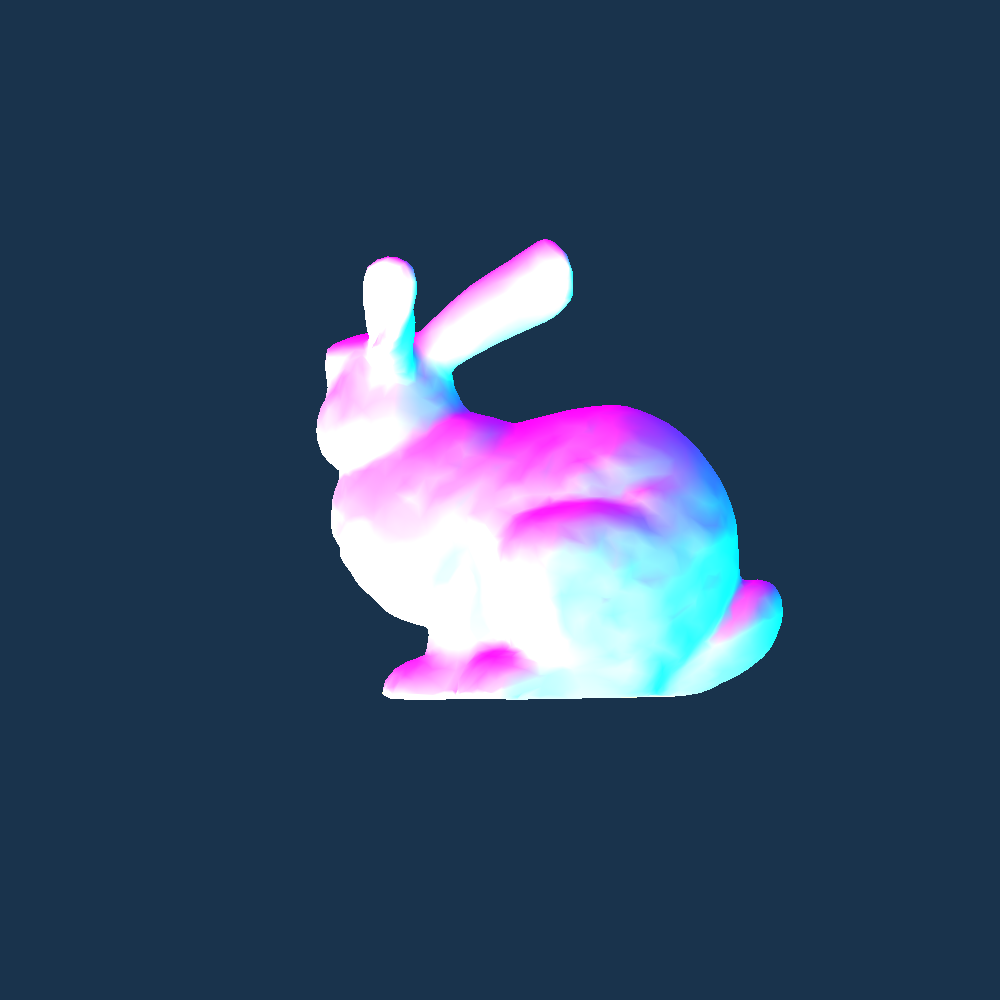
\includegraphics[width=0.4\textwidth]{fig/fig1.png}
	\caption{Bunny1}
	\label{Bunny1}
\end{figure}

\subsection{Render objects with a Phong lighting model}
I created 3 light sources with red, green, and blue color.
And they rotate constantly on XY, XZ, and YZ planes.
\begin{figure}[htb]
	\centering
	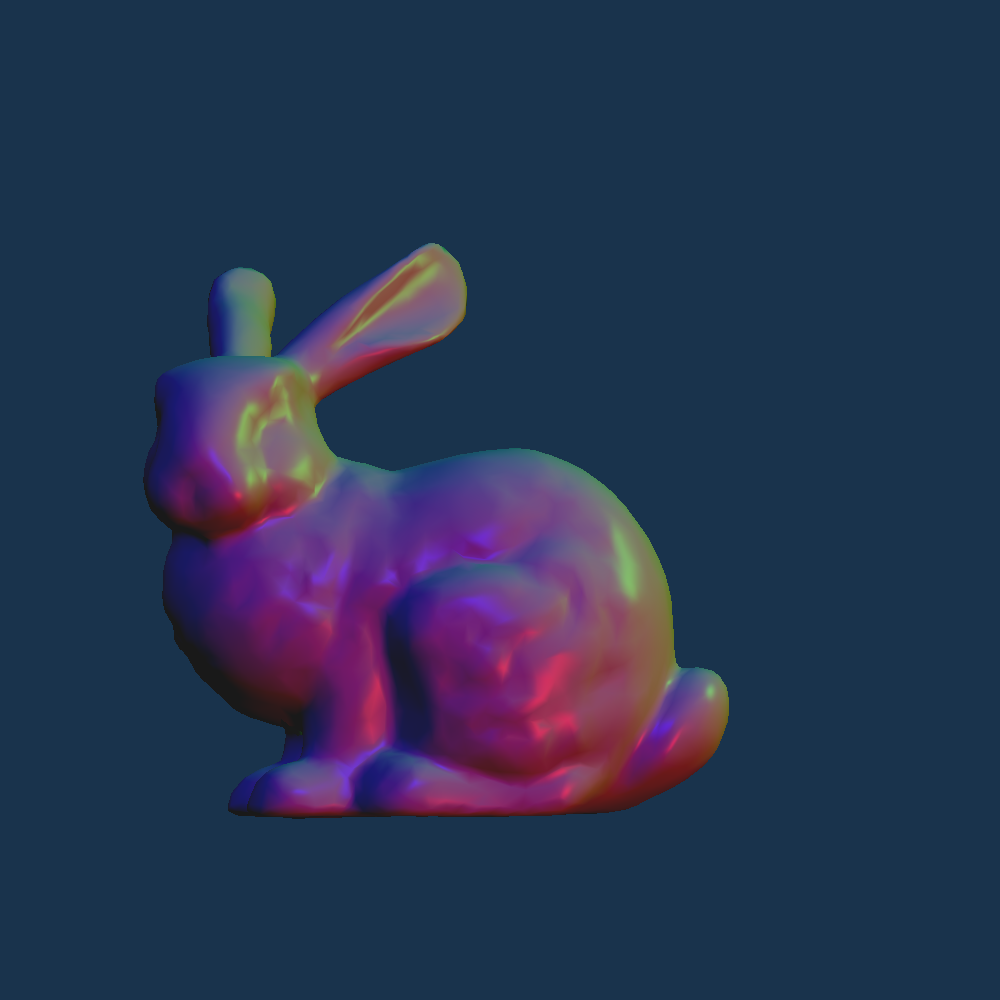
\includegraphics[width=0.4\textwidth]{fig/fig2.png}
	\caption{Bunny2}
	\label{Bunny2}
\end{figure}

\newpage
\subsection{Camera and controlling}
Another view of Bunny.
\begin{figure}[htb]
	\centering
	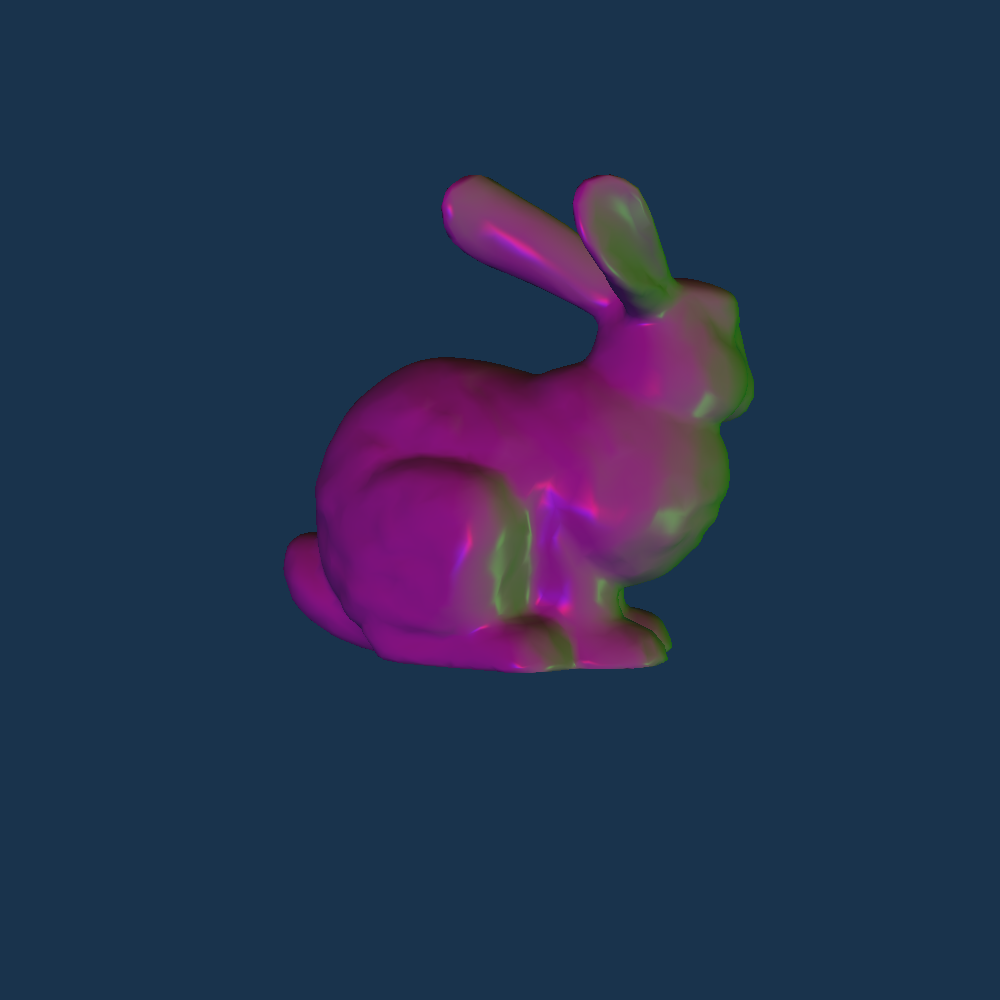
\includegraphics[width=0.4\textwidth]{fig/fig3.png}
	\caption{Bunny3}
	\label{Bunny3}
\end{figure}


\end{document}
